\selectlanguage{italian}
\graphicspath{ {img/4/} }
\chapter{Viola Jones e Haar Cascades}\label{cap:ViolaHaar}
\thispagestyle{empty} %Elimina il numero della prima pagina del capitolo.
\newpage

\section{Viola Jones}
\vspace{8mm}

La classificazione delle immagini è un campo in rapida crescita e l'utilizzo delle reti neurali convoluzionali (CNN) e di altre tecniche di apprendimento è in rapida crescita.
Tuttavia, prima che le CNN diventassero di utilizzo comune, un'altra tecnica era ampiamente utilizzata e continua ad essere utilizzata: \emph{Viola-Jones}.
Mentre una CNN è un singolo classificatore che osserva un'immagine per intero e applica operazioni matriciali per arrivare a una classificazione, Viola-Jones adotta un approccio d'insieme. Ciò significa che Viola-Jones utilizza molti classificatori diversi, ognuno dei quali osserva una diversa porzione dell'immagine. Ogni singolo classificatore è più debole (meno accurato, produce più falsi positivi) rispetto al classificatore finale perché riceve meno informazioni. Quando i risultati di ciascun classificatore vengono combinati, tuttavia, viene prodotto un classificatore forte.

\begin{figure}[h!]
	\centering
	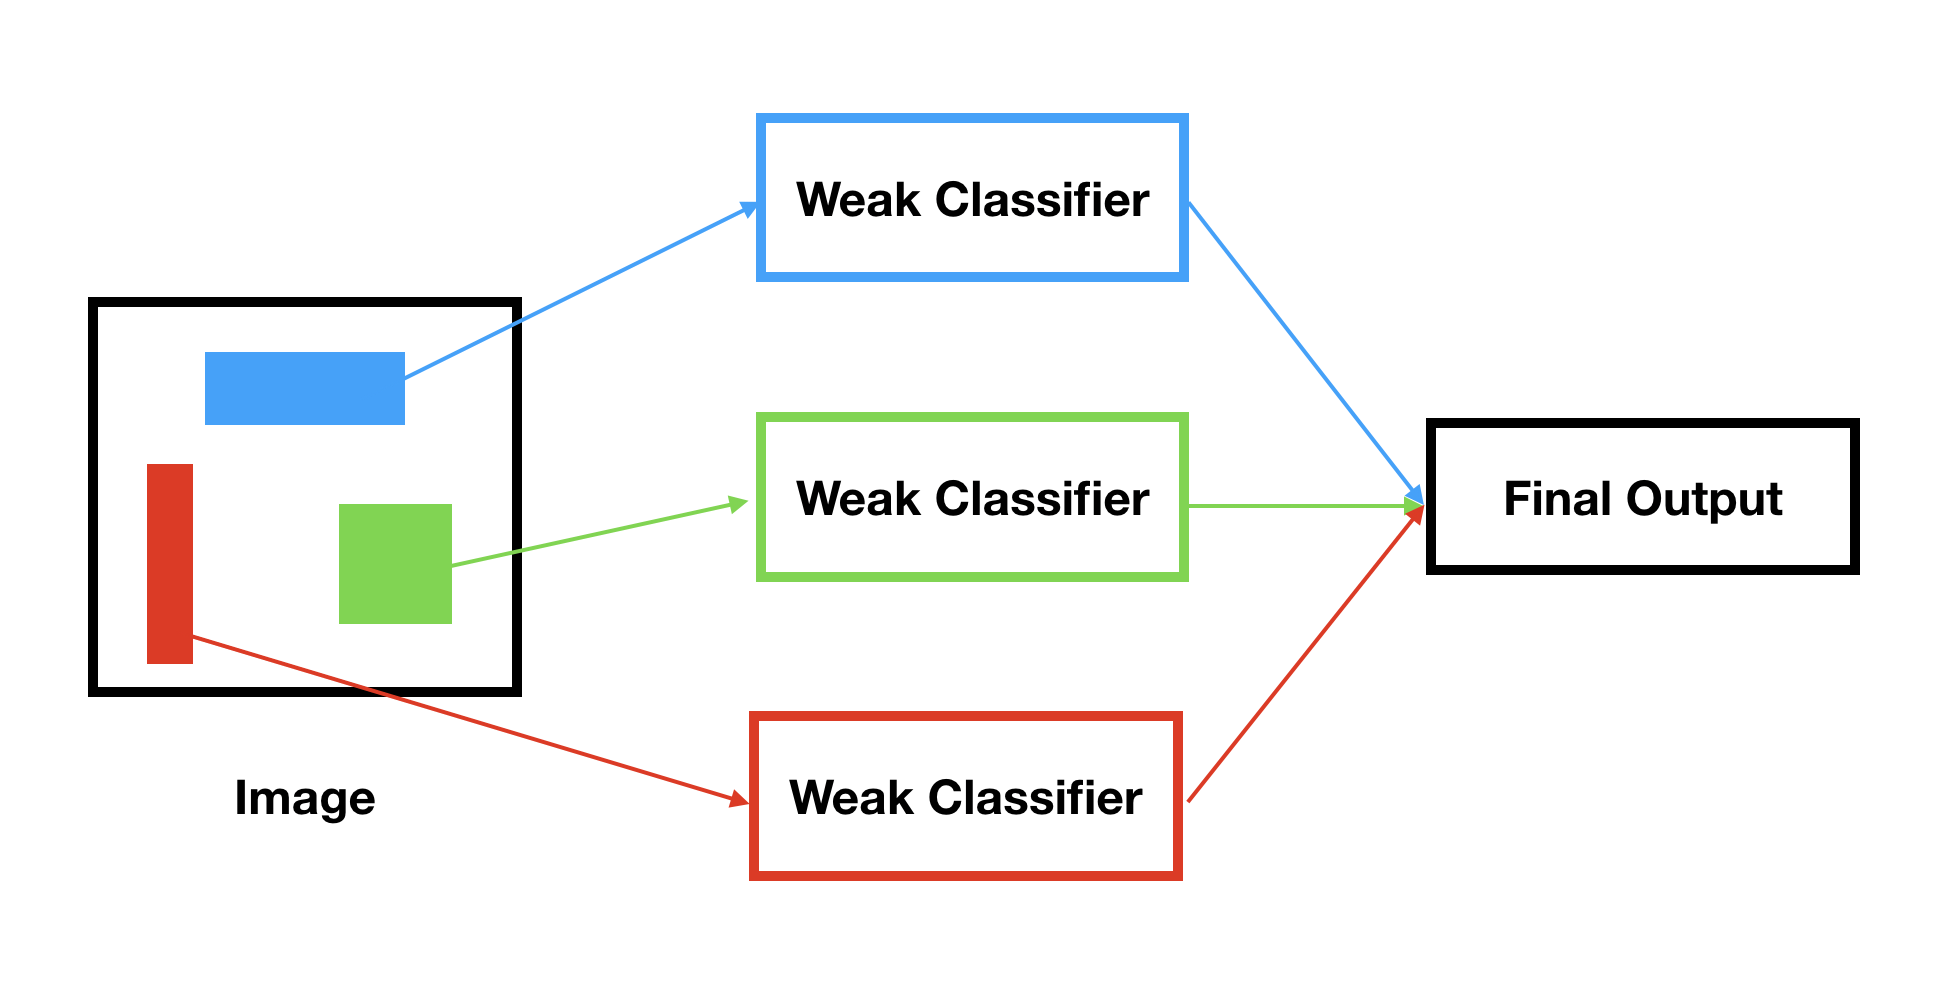
\includegraphics[width=80mm]{img/4/violahaar_1_1}
	\caption{\fontsize{10px}{0mm}\selectfont Classificatori in Viola-Jones \label{fig:violahaar_1_1}}
\end{figure}

A causa della natura dell'algoritmo, il metodo Viola-Jones è limitato alle attività di classificazione binaria (come il rilevamento di oggetti) e ha un periodo di training piuttosto lungo. Tuttavia, esso classifica le immagini rapidamente grazie al fatto che ogni classificatore debole richiede solo un piccolo numero di parametri, inoltre, con un numero sufficiente di classificatori deboli, l'algoritmo ha un basso tasso di falsi positivi\footnote{Un falso positivo è un risultato in cui il modello prevede erroneamente la classe come positiva.}.
\newpage
\subsection{Features e Integral Image}
Uno dei primi contributi chiave apportati nel documento\cite{violapaper} che introduce Viola-Jones è stato un insieme di semplici feature da utilizzare nel riconoscimento delle immagini. Nella maggior parte delle attività, i valori dei pixel sono le caratteristiche immesse nell'algoritmo. Tuttavia, Viola e Jones hanno introdotto le seguenti nuove feature.

\begin{figure}[h!]
	\centering
	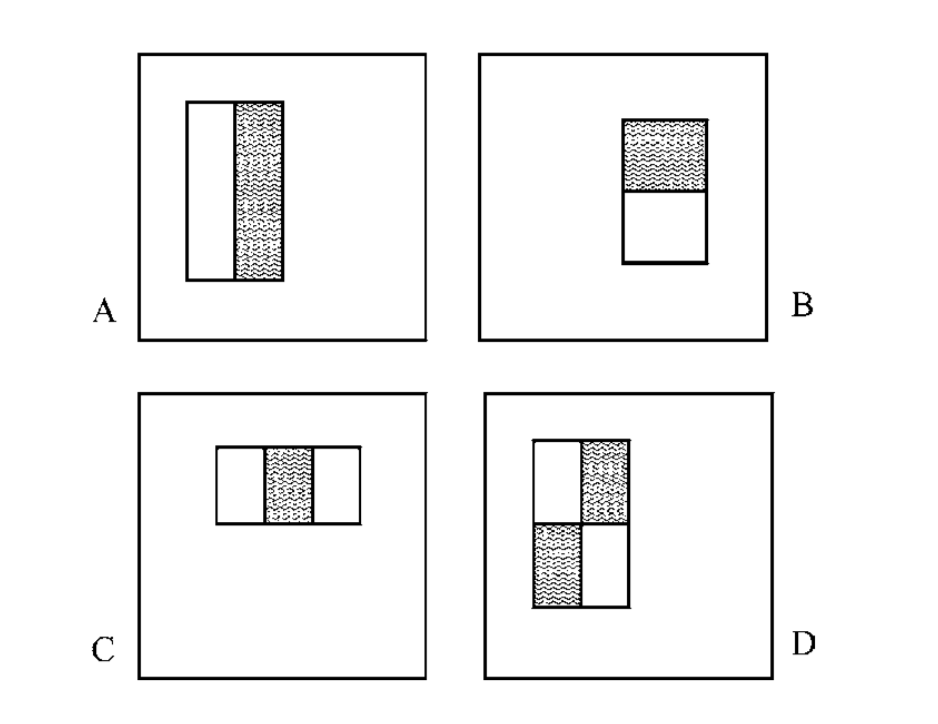
\includegraphics[width=80mm]{img/4/violahaar_1_2}
	\caption{\fontsize{10px}{0mm}\selectfont A e B sono feature a due rettangoli, C è una feature a tre rettangoli e D è una feature a 4 rettangoli. Immagine tratta dal documento originale. \label{fig:violahaar_1_2}}
\end{figure}

La somma dei pixel nei rettangoli non ombreggiati viene sottratta dalla somma dei pixel nei rettangoli ombreggiati. È facile vedere che anche per le immagini di piccole dimensioni ci sono molte feature (oltre 160.000 per un'immagine 24 x 24). Poiché l'algoritmo richiede l'iterazione di tutte le feature, è necessario calcolarle in modo molto efficiente. Per fare questo, Viola e Jones hanno introdotto le \emph{Integral Image}, L'immagine integrale è definita dalla seguente relazione ricorsiva: \newpage

\begin{figure}[h!]
	\centering
	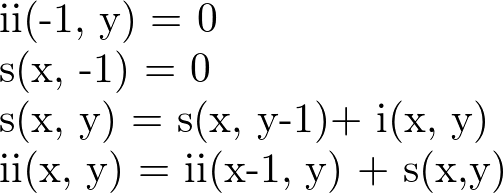
\includegraphics[width=80mm]{img/4/violahaar_1_3}
	\caption{\fontsize{10px}{0mm}\selectfont Relazione ricorsiva dell'immagine integrale \label{fig:violahaar_1_3}}
\end{figure}
$s(x, y)$ è la somma cumulativa delle righe nel punto $(x, y)$, $ii(x, y)$ è il valore dell'immagine integrale nello stesso punto e $i(x, y)$ è il valore del pixel in quel punto. Questa relazione non dice altro che l'immagine integrale in un punto $(x, y)$ è la somma di tutti i pixel in alto a sinistra rispetto al pixel corrente. Ciò semplifica il calcolo della somma dei pixel in una regione rettangolare come mostrato di seguito.


\begin{figure}[h!]
	\centering
	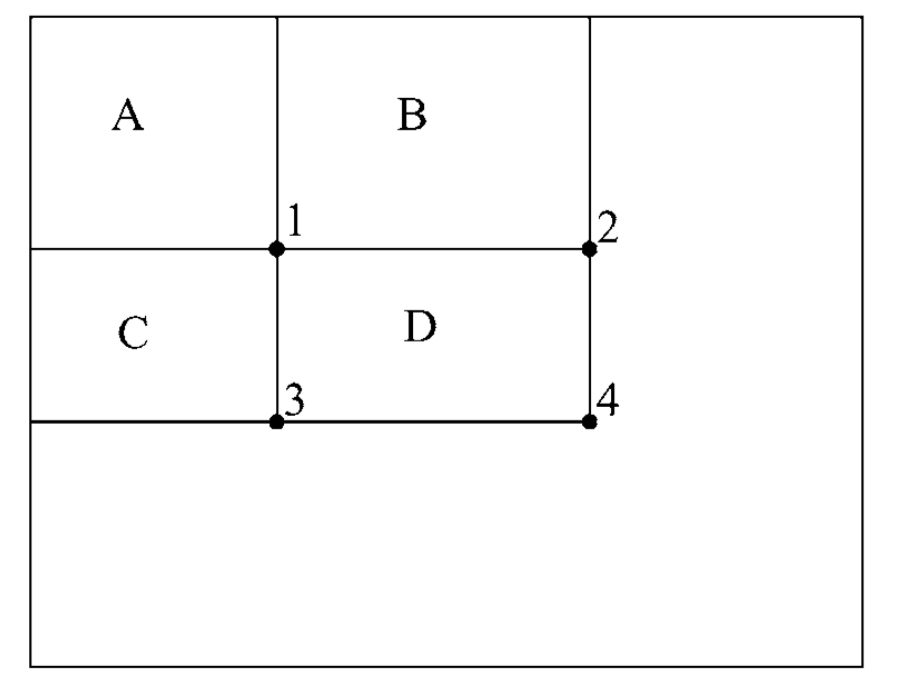
\includegraphics[width=80mm]{img/4/violahaar_1_4}
	\caption{\fontsize{10px}{0mm}\selectfont Calcolo dei pixel in una regione rettangolare \label{fig:violahaar_1_4}}
\end{figure}

La somma dei pixel nella regione $D$ è $ii(4) + ii (1) - ii (2) - ii (3)$ che non sono altro che quattro riferimenti ad array.\newpage

\subsection{Training e Weak Classifiers}

Il ciclo principale di training richiede la scelta del miglior classificatore debole, ma esiste un classificatore debole per ogni possibile caratteristica. Per questo motivo, dobbiamo creare tutte le feature prima di iniziare a implementare il ciclo principale di training.

Quando verranno identificati i classificatori deboli ottimali da utilizzare in seguito nell'algoritmo, sarà necessario valutare ciascuna feature per ogni esempio di training. Per risparmiare computazione, verrà effettuata la valutazione di ogni feature prima di iniziare il training dei classificatori. Questa scelta è più efficiente perché ogni classificatore deve essere riqualificato ogni volta che ne viene selezionato uno nuovo.

Viola-Jones utilizza una serie di classificatori deboli e pondera i loro risultati insieme per produrre la classificazione finale. Ogni classificatore è "debole" perché da solo non può adempiere con precisione all'attività di classificazione. Ogni classificatore debole osserva una singola feature $f$, ha una soglia $\theta$ e una polarità $p$ per determinare la classificazione di un esempio di training.
\begin{figure}[h!]
	\centering
	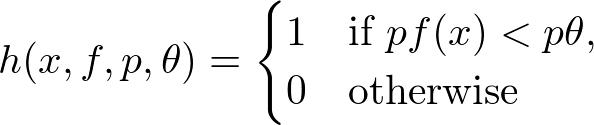
\includegraphics[width=80mm]{img/4/violahaar_1_5}
	\caption{\fontsize{10px}{0mm}\selectfont Classificatore debole \label{fig:violahaar_1_5}}
\end{figure}

La polarità può essere -1 o 1. Quando $p=1$, il classificatore debole produce un risultato positivo quando $f(x)<\theta$ o quando il valore della feature è inferiore alla soglia. Quando $p=-1$ il classificatore debole produce un risultato positivo per $f(x)>\theta$.\newpage

Si noti che ogni feature è la somma delle regioni rettangolari positive con la somma delle regioni rettangolari negative sottratte da esse. Il prossimo passo dell'algoritmo è scegliere il miglior classificatore debole. Per fare ciò, dobbiamo trovare la soglia e la polarità ottimali per ognuno di essi.

L'addestramento dei classificatori deboli è la parte più costosa dal punto di vista computazionale dell'algoritmo. Ogni volta che un nuovo classificatore debole viene selezionato come il migliore, tutti gli altri devono essere riqualificati poiché gli esempi di allenamento sono pesati in maniera diversa. Tuttavia, esiste un modo efficiente per trovare la soglia e la polarità ottimali per un singolo classificatore debole utilizzando i pesi. Innanzitutto, si ordinano i pesi in base al valore della feature alla quale corrispondono, dopodiché si scorre attraverso la matrice dei pesi e si calcola l'errore se la soglia è stata scelta per essere quella feature. Infine, si trovano soglia e polarità aventi il minimo errore. I possibili valori per una soglia sono i valori della feature su ciascun esempio di allenamento. L'errore può essere misurato da:

$$ e = \min{(S^+ + T^- - S^-, S^- + T^+ - S^+)} $$

Dove $T$ rappresenta la somma totale dei pesi e $S$ rappresenta la somma dei pesi di tutti gli esempi visti finora. Gli apici $+$ e $-$ indicano a quale classe appartiene la somma. Concettualmente, questo errore confronta quanti esempi verranno classificati in modo errato se tutti gli esempi al di sotto della posizione corrente sono etichettati come negativi con quanti esempi saranno classificati in modo errato se tutti gli esempi al di sotto della posizione corrente sono etichettati come positivi (tenendo conto di come ogni esempio è pesato).

In questa maniera, è possibile valutare l'errore di ogni possibile soglia in tempo costante $(O(1))$ e l'errore di tutte le soglie in tempo lineare $(O(n))$. La soglia è impostata sul valore della feature per cui l'errore è minimo. La polarità è determinata da quanti esempi positivi ed esempi negativi si trovano a sinistra (minore) e a destra(maggiore) della soglia. Se rimangono altri esempi positivi a sinistra della soglia allora $p=1$. Altrimenti, $p=-1$.

\begin{figure}[h!]
	\centering
	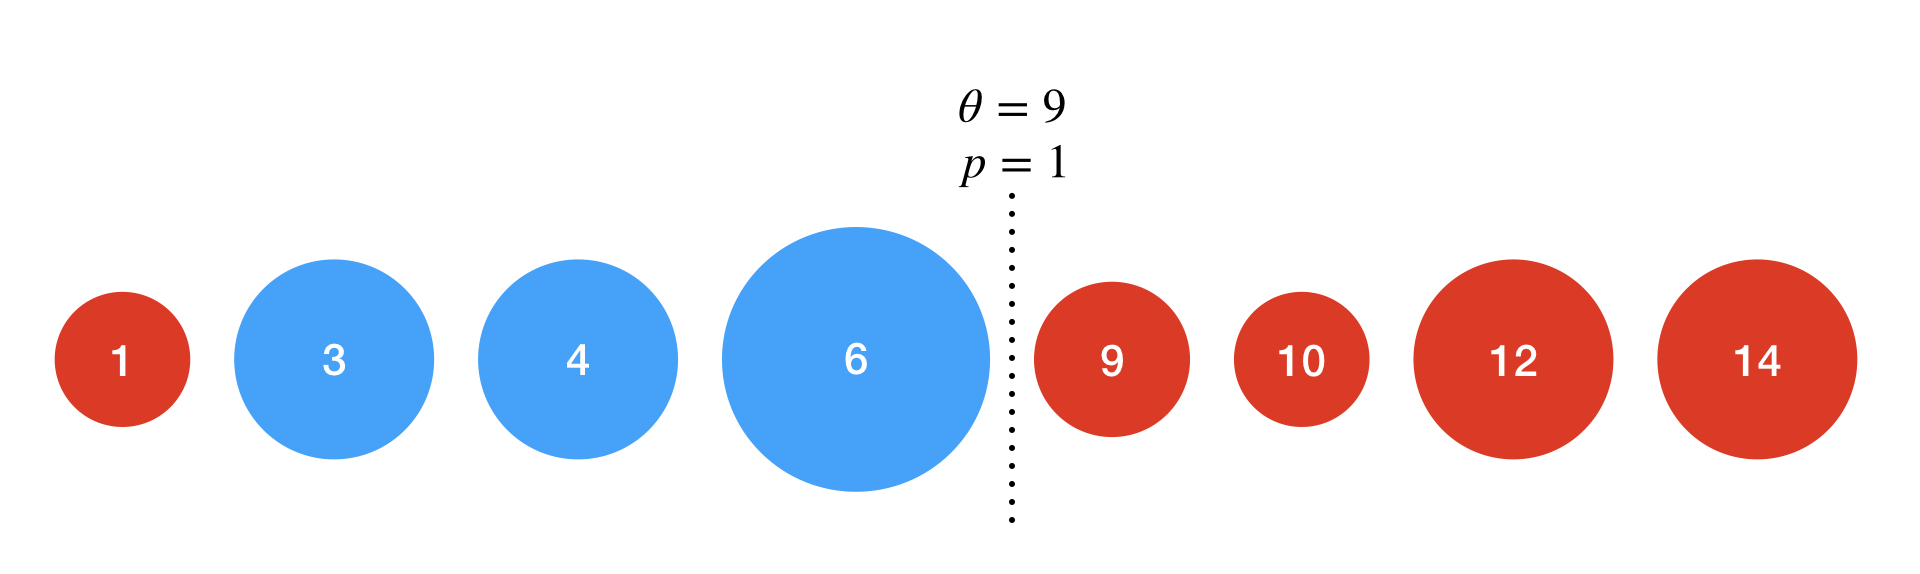
\includegraphics[width=100mm]{img/4/violahaar_1_6}
	\caption{\fontsize{10px}{0mm}\selectfont In questo esempio, i numeri indicano i valori delle feature e la dimensione delle bolle indica i loro pesi relativi. Chiaramente, l'errore verrà minimizzato quando qualsiasi feature con un valore inferiore a 9 viene classificata come blu. Ciò corrisponde a una soglia di 9 con una polarità di 1. \label{fig:violahaar_1_6}}
\end{figure}
Una volta addestrati tutti i classificatori deboli, possiamo trovare il migliore semplicemente scorrendo attraverso tutti i classificatori e calcolando l'errore medio pesato di ciascuno di essi.\newpage

\subsection{Strong Classifier}
L'ultimo passaggio riguarda il classificatore finale. Dobbiamo compilare il classificatore forte a partire dai classificatori deboli. Il classificatore forte è definito come:

\begin{figure}[h!]
	\centering
	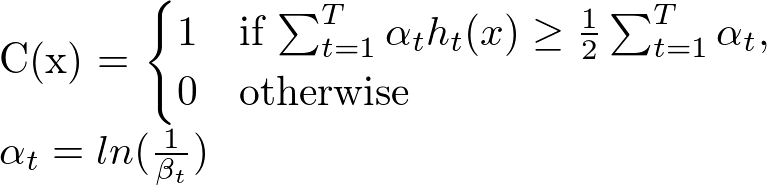
\includegraphics[width=100mm]{img/4/violahaar_1_7}
	\caption{\fontsize{10px}{0mm}\selectfont Definizione classificatore forte \label{fig:violahaar_1_7}}
\end{figure}


Il coefficiente $\alpha$ indica quanto ciascun classificatore debole è rilevante nella decisione finale e dipende dall'errore poiché è il logaritmo naturale dell'inverso di $\beta$. La somma pesata delle decisioni dei classificatori deboli viene confrontata con la metà della somma degli $\alpha$.
\cite{violajones}

\section{Considerazioni riguardanti Viola-Jones}
\vspace{8mm}
In base a quanto descritto finora, la struttura dell'algoritmo di classificazione Viola-Jones rende l'approccio particolarmente robusto sia per la selezione di feature che per la classificazione di immagini. Il documento originale di Viola-Jones introduce vari concetti per ridurre il tempo di classificazione.
Durante la fase di progettazione, quindi, sono state considerate diverse opzioni per ottimizzare l'algoritmo e rendere l'approccio quanto più performante possibile soprattutto in base alle considerazioni descritte nella sezione \ref{considerazioniCNN} riguardanti la mancanza e l'estrema specificità dei dati.
\newpage

\section{Haar Cascades}
\vspace{8mm}

Haar Cascades è un algoritmo di Machine Learning utilizzato per identificare oggetti in un'immagine o in un video. È basato sul concetto di feature proposto da Paul Viola e Michael Jones nel loro articolo "Rapid Object Detection using a Boosted Cascade of Simple Features" nel 2001. L'idea è che viene utilizzata una funzione a cascata, addestrata a partire da immagini positive e negative. Viene utilizzato quindi per rilevare oggetti all'interno di immagini. È noto per essere in grado di rilevare volti e parti del corpo in un'immagine, ma può essere addestrato per identificare quasi qualsiasi oggetto.
\\
L'algoritmo è composto da 4 fasi:

\begin{enumerate}
  \item Haar Feature Selection
  \item Creating Integral Images
  \item Adaboost Training
  \item Cascading Classifiers
\end{enumerate}

\subsection{Haar Feature e Adaboosting}
Prendiamo il rilevamento del volto come esempio. Inizialmente, l'algoritmo necessita di immagini positive di volti e immagini negative senza volti per addestrare il classificatore. Quindi dobbiamo estrarre feature da esso.\newpage

Il primo passo è quello di raccogliere le \emph{Haar Features}. Una Haar Feature considera le regioni rettangolari adiacenti in una posizione specifica in una finestra di rilevamento, somma le intensità dei pixel in ciascuna regione e calcola la differenza tra queste somme. Per rendere questo procedimento molto rapido, vengono utilizzate le \emph{Integral Image}
\begin{figure}[h!]
	\centering
	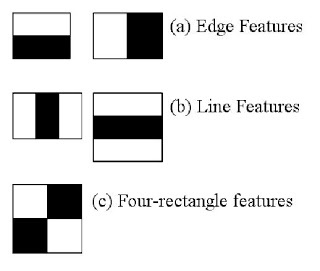
\includegraphics[width=80mm]{img/4/violahaar_1_8}
	\caption{\fontsize{10px}{0mm}\selectfont Haar Feature \label{fig:violahaar_1_8}}
\end{figure}

Si noti che la maggior parte delle feature calcolate è irrilevante. Si consideri l'immagine riportata in seguito. La riga superiore mostra due feature rilevanti. La prima feature selezionata sembra concentrarsi sulla proprietà che la regione degli occhi è spesso più scura della regione del naso e delle guance. La seconda feature selezionata si basa sulla proprietà che gli occhi sono più scuri del ponte del naso. Contemporaneamente, però, le stesse finestre che si applicano sulle guance o in qualsiasi altro posto sono irrilevanti.

\begin{figure}[h!]
	\centering
	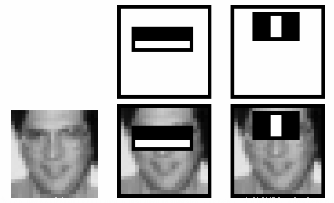
\includegraphics[width=60mm]{img/4/violahaar_1_9}
	\caption{\fontsize{10px}{0mm}\selectfont Esempio di Haar Feature \label{fig:violahaar_1_9}}
\end{figure} \newpage


Come possiamo selezionare le migliori funzionalità tra le oltre 160.000 funzionalità? La risposta a tale domanda risiede in un approccio chiamato \emph{Adaboost}, che seleziona le migliori feature e addestra i classificatori che le usano. Questo algoritmo costruisce un classificatore “forte” come una combinazione lineare di classificatori “deboli” pesati. Il processo è il seguente:

Durante la fase di rilevamento, una finestra della dimensione del target viene spostata sull'immagine di input e per ciascuna sottosezione dell'immagine vengono calcolate le Haar Feature.
Questa differenza viene successivamente confrontata con una soglia appresa che separa gli oggetti della classe di oggetti di interesse da quelli che non vi appartengono. Poiché ogni Haar Feature è solo un "classificatore debole" (la sua qualità di rilevazione è leggermente migliore di una supposizione casuale) è necessario un gran numero di Haar Feature per descrivere un oggetto con sufficiente precisione, di conseguenza si organizzano le Haar Feature in \emph{Cascade Classifiers}(classificatori a cascata) per formare un classificatore forte.

\subsection{Cascade Classifier}

Il classificatore a cascata è costituito da una raccolta di fasi, in cui ogni fase è un insieme di \emph{Weak Learner}. I Weak Learner sono semplici classificatori chiamati \emph{decision stumps}. Per ogni fase il training avviene utilizzando una tecnica nota come \emph{boosting}. Il boosting fornisce la capacità di addestrare un classificatore altamente accurato prendendo una media ponderata delle decisioni prese dai classificatori deboli.

Ogni fase del classificatore identifica la regione definita dalla posizione corrente della finestra scorrevole come positiva o negativa. Positivo indica che è stato trovato un oggetto e negativo indica che non sono stati trovati oggetti. 

Se l'etichetta è negativa, la classificazione di questa regione è completa e il rilevatore fa scorrere la finestra nella \emph{posizione} successiva. Se l'etichetta è positiva, il classificatore passa la regione alla \emph{fase} successiva. Il rilevatore segnala un oggetto trovato nella posizione corrente della finestra quando la fase finale classifica la regione come positiva.

Le fasi sono progettate per rifiutare campioni negativi il più rapidamente possibile. L'ipotesi è che la stragrande maggioranza delle finestre non contenga l'oggetto di interesse. Al contrario, i \emph{true positive} sono rari e vale la pena dedicare del tempo alla verifica.
\begin{itemize}
  \item Un \textbf{true positive} si verifica quando un campione positivo è correttamente classificato.
  \item Un \textbf{false positive} si verifica quando un campione negativo viene erroneamente classificato come positivo.
  \item Un \textbf{false negative} si verifica quando un campione positivo viene erroneamente classificato come negativo.
\end{itemize}

Per un corretto funzionamento, ogni fase della cascata deve avere un basso tasso di false negative. Se una fase etichetta erroneamente un oggetto come negativo, la classificazione si interrompe e non è possibile correggere l'errore. Tuttavia, ogni fase può avere un alto tasso di falsi positivi. Anche se il rilevatore etichetta erroneamente un non-oggetto come positivo, è possibile correggere l'errore nelle fasi successive. L'aggiunta di più fasi riduce il tasso complessivo di false positive, ma riduce anche il tasso complessivo di true positive.

Il training del classificatore a cascata richiede una serie di campioni positivi e una serie di immagini negative. È necessario fornire una serie di immagini positive con le regioni di interesse specificate che verranno utilizzate come campioni positivi. È inoltre necessario fornire un set di immagini negative da cui la funzione genera automaticamente campioni negativi.
\cite{haarcascades}\newpage


\section{Considerazioni riguardanti Haar Cascades}
\vspace{8mm}

In base a quanto descritto nelle precedenti sezioni, un approccio basato sull'algoritmo Haar Cascades può portare ottime prestazioni se utilizzato in maniera corretta.
Rispetto all'approccio basato su Viola-Jones, Haar Cascades si presta più efficiente e più fluido in task di rilevazione di individui \emph{in qualsiasi contesto}.
Nel prossimo capitolo viene mostrato come Haar Cascades è stato utilizzato nella stesura del software.
\newpage